\documentclass[12pt, a4paper]{report}

% --- Inclusion des configurations ---
% Load project-specific settings first so packages/layout can reuse them
% =====================================
% VARIABLES SPÉCIFIQUES AU PROJET
% =====================================

% --- Commandes modulaires pour le rapport (À MODIFIER POUR CHAQUE PROJET) ---
\newcommand{\authorA}{VIRQUIN Rudy}
\newcommand{\authorB}{}
% Inline authors used for headers (comma-separated)
\newcommand{\authorsInline}{\authorA}

\newcommand{\documentTitle}{PROJET GE S8}
\newcommand{\documentSubtitle}{La petite maison dans la prairie}
\newcommand{\documentSubject}{RAPPORT 1}

% Backwards-compatible names used elsewhere in the project
\newcommand{\tpnumero}{}
\newcommand{\tptitre}{\documentTitle}
\newcommand{\tpsoustitre}{\documentSubtitle}
\newcommand{\tpmatiere}{\documentSubject}
\newcommand{\tpauteurs}{%
	\begin{tabular}{c}
		\authorA
	\end{tabular}
}
\newcommand{\tpgroupe}{}
\newcommand{\tpprofesseur}{Jean-Michel Hube et Bertrand Boyer}
\newcommand{\tpdate}{\today}


% --- Page de garde personnalisée ---
\newcommand{\maketitlepage}{
    \begin{titlepage}
        \centering
        
\includegraphics[width=0.5\textwidth]{images/logo_insa.jpg}\par\vspace{1cm}
        {\Huge\bfseries \tptitre\par}
        \vspace{1.5cm}
        {\huge\bfseries \tpsoustitre\par}
        \vspace{2cm}
        {\Large\itshape \tpauteurs\par}
        {\Large\itshape Groupe 2 \tpgroupe\par}
        \vspace{2cm}
        {\begin{figure}[H]
    \centering
    \begin{tikzpicture}[scale=1.5, transform shape]
	% Paths, nodes and wires:
	\node[nigfete] at (8.98, 7.27){};
	\draw (9.48, 6.5) to[empty diode, l_={$T$}] (9.48, 8.04);
	\draw (9.48, 8.04) -| (8.98, 8.04);
	\draw (9.48, 6.5) -- (8.98, 6.5);
	\node[ieeestd buffer port](N1) at (7.152, 7){} node[anchor=south] at ([yshift=0.05cm]N1.north){$Driver$};
	\draw (2, 10) to[european voltage source, l={$24\mathrm{V}$}] (2, 6);
	\draw (4, 10) to[capacitor, l^={$C_{Découplage}$}] (4, 8);
	\draw (6.275, 7) to[square voltage source, l_={$GBF$}] (4, 7);
	\draw (4, 8) -- (4, 7);
	\node[ground] at (4, 6){};
	\draw (4, 7) -| (4, 6) -| (8.98, 6.5);
	\draw (8, 8.667) to[empty diode] (8, 10);
	% Remplacer le composant unique "RL" par une résistance et une inductance en série
	% on découpe le segment vertical en deux parties et on place R puis L
	\draw (9, 8.667)  to[L, l_={$RL$}] (9, 10);
	\draw (8.98, 8.04) -| (9, 8.667);
	\draw (8, 8.667) -- (9, 8.667);
	\draw (4, 6) -- (2, 6);
	\draw (2, 10) -- (8, 10);
	\draw (8, 10) -- (9, 10);
	\node[circ] at (4, 10){};
	\node[circ] at (4, 7){};
	\node[circ] at (4, 6){};
	\node[circ] at (9, 8.667){};
	\node[circ] at (8, 10){};
\end{tikzpicture}
\end{figure}}
        \vfill
        {\large Professeur : \tpprofesseur\par}
        \vspace{0.8cm}
        {\large \tpdate\par}
    \end{titlepage}
} % Variables du projet
% =====================================
% CONFIGURATION DES PACKAGES ET COULEURS
% =====================================

% --- Encodage et langue ---
\usepackage[utf8]{inputenc}
\usepackage[T1]{fontenc}
\usepackage[french]{babel}
\renewcommand{\familydefault}{\sfdefault}  % Utilise Computer Modern Sans Serif
\renewcommand{\sfdefault}{qag}  % Spécifie cmss comme police sans empattement

% --- Package pour une meilleure justification ---
\usepackage{ragged2e}
\justifying  % Active la justification par défaut

% --- Packages pour la mise en page et le contenu ---
\usepackage{graphicx}   %% Pour inclure des images
\usepackage{pdfpages}   %% Pour inclure des pages PDF entières

% Configuration pour trouver les images (compatible LaTeX Workshop + Overleaf)
% Le chemin doit finir par / et être entre accolades
\graphicspath{{./images/}{images/}{../Rapport/images/}}

\usepackage[a4paper]{geometry} % Gestion des marges
% Configuration des marges ET des espaces pour l'en-tête/pied de page
\geometry{
  left=2cm,        % Marge gauche (augmentez pour "agrandir")
  right=2cm,       % Marge droite (augmentez pour "agrandir")
  top=2.5cm,         % Marge haute (augmentez pour "agrandir")
  bottom=1.5cm,      % Marge basse (augmentez pour "agrandir")
  headheight=34pt, % Indique à geometry la taille de votre en-tête fancyhdr
  footskip=24pt,    % Indique à geometry l'espace pour votre pied de page
  headsep=0.5cm
}

\usepackage{amsmath, amssymb}       % Outils mathématiques avancés
% Numérotation continue des équations : 1,2,3... (sans préfixe chapitre)
\usepackage{chngcntr}
\counterwithout{equation}{chapter}
\renewcommand{\theequation}{\arabic{equation}}
\usepackage[
    hidelinks,
    pdftitle={\documentTitle},
    pdfauthor={\authorA, \authorB},
    pdfsubject={\documentSubject},
    pdfkeywords={électronique de puissance, cellule de commutation, INSA Strasbourg, ENPU2},
    pdfcreator={LaTeX},
    pdfproducer={LaTeX}
]{hyperref}    % Pour les liens cliquables et métadonnées PDF
\usepackage{fancyhdr}               % Pour personnaliser les en-têtes et pieds de page
\usepackage{xcolor}                 % Pour utiliser des couleurs
\usepackage{tcolorbox}              % Pour créer des boîtes colorées
\usepackage{float}                  % Pour mieux placer les figures
\usepackage{newfloat}              % Pour créer des environnements flottants personnalisés
\usepackage{caption}                % Pour personnaliser les légendes
\usepackage{subcaption}             % Pour des sous-figures
\usepackage{etoolbox}              % Pour hook AtBeginEnvironment
% --- Style personnalisé pour les légendes des tableaux ---
% On veut : petite taille, largeur limitée à la largeur de la table,
% possibilité de plusieurs lignes et fond gris clair.
\DeclareCaptionFont{smallit}{\tiny}
% Define a caption format that places the caption text inside a colored box
% whose width is the caption width (which will be set to the table width).
% Draw a gray background with a black frame that matches the caption width.
% We account for the frame thickness (\fboxrule) and padding (\fboxsep) so the outer
% \fcolorbox total width equals the requested caption width (which is \linewidth inside
% the caption context). The inner parbox width is therefore \linewidth - 2\fboxrule - 2\fboxsep.
\DeclareCaptionFormat{graybox}{%
        {%
                % Use local settings for border thickness and padding. We'll use \arrayrulewidth
                % as the default border width for consistency with table rules.
                \setlength{\fboxrule}{\arrayrulewidth}%
                \setlength{\fboxsep}{0.5pt}% small inner padding so the gray fills to the border
                % Compute inner width; if \dimexpr is available this will evaluate safely here.
                \begingroup
                    \colorlet{captionframe}{black}% frame color
                    \colorlet{captionbg}{boxgray}% background color
                    \edef\innerwidth{\the\dimexpr\linewidth-2\fboxrule-2\fboxsep\relax}%
                    \fcolorbox{captionframe}{captionbg}{% outer framed box (total width = \linewidth)
                        \parbox{\innerwidth}{% inner box sized so outer frame equals \linewidth
                            \hspace{0.15em}#1#2#3\hspace{0.15em}% small horizontal padding
                        }% end parbox
                    }% end fcolorbox
                \endgroup
        }%
}
% Apply the format to table captions: smaller font, the graybox format,
% allow multi-line captions and left-aligned wrapping. We do NOT hardcode a
% global width here because \linewidth at package load time is the text width,
% not the float width. Instead, ensure that at the start of every table float
% we set the caption width to the current \linewidth (i.e. the table width).
\captionsetup[table]{format=graybox,font=smallit,labelfont=bf}
% When entering a table environment, set caption width to the current \linewidth
% so the caption box will match the table's width.
\AtBeginEnvironment{table}{\captionsetup{width=\linewidth}}
% Reduce the vertical gap between table and caption and force label on its own line
\setlength{\abovecaptionskip}{0pt}
\setlength{\belowcaptionskip}{0pt}
\captionsetup[table]{format=graybox,font=smallit,labelfont=bf,justification=raggedright,singlelinecheck=false,margin=0pt,labelsep=newline,skip=0pt}

% --- Configuration des légendes pour les figures ---
% Réduction de la taille de police pour les captions de figures
\captionsetup[figure]{font=small,labelfont=bf,justification=centering}

% --- Nouvel environnement 'tableau' pour tableaux sans style spécial ---
% Création d'un nouvel environnement flottant nommé 'tableau'
\DeclareFloatingEnvironment[
    fileext=lot,        % Utilise la même liste que les tables
    listname={Liste des tableaux},
    name=Tableau,
    placement=tbp,      % Placement par défaut : top, bottom, page
    within=none         % Numérotation continue dans tout le document
]{tableau}

% Configuration du caption pour l'environnement 'tableau' : style simple, sans boîte grise
\captionsetup[tableau]{
    format=plain,           % Format simple sans boîte
    font=small,             % Taille de police normale (pas tiny)
    labelfont=bf,           % Label en gras
    justification=centering, % Centré
    singlelinecheck=true,   % Permet le centrage automatique pour les légendes courtes
    margin=0pt,
    labelsep=colon,         % Séparateur standard "Tableau X:"
    skip=10pt               % Espacement normal entre tableau et caption
}

% Optional helper environment: tablebox
% Usage: \begin{table}\begin{tablebox}{<width>} ... \end{tablebox}\end{table}
% This wraps content in a minipage so that \linewidth inside equals <width>
\newenvironment{tablebox}[1][\linewidth]{%
    \begin{minipage}{#1}
}{%
    \end{minipage}
}
\usepackage{booktabs}               % Pour de jolis tableaux
% Allow tables that stretch to a target width
\usepackage{tabularx}
\usepackage{array}
% Right-aligned X column for tabularx
\newcolumntype{R}{>{\raggedleft\arraybackslash}X}
\usepackage{titlesec}               % Pour personnaliser les titres de chapitres
\usepackage{lastpage}               % Pour obtenir le nombre total de pages
\usepackage{datetime}               % Pour le formatage des dates
\usepackage{pgfplots}
% Ensure pgfplots uses modern compatibility level to avoid backward-compatibility warnings
\pgfplotsset{compat=1.18}

% Package for placing content absolutely on the page background/foreground
\usepackage{eso-pic}

% --- Package CircuiTikz avec configuration spéciale ---
\usepackage{tikz}                   % TikZ doit être chargé avant circuitikz
\usepackage[siunitx]{circuitikz} % Configuration pour les diagrammes électriques
\usetikzlibrary{babel, positioning, shapes, arrows, patterns} % Bibliothèques TikZ supplémentaires

% --- Définition des couleurs personnalisées ---
\definecolor{INSAbleu}{RGB}{0, 70, 127}
\definecolor{INSArouge}{RGB}{229, 39, 19}
\definecolor{boxgray}{gray}{0.95}
\definecolor{remindercolor}{RGB}{96, 98, 103}     % gris INSA pour les rappels
% Couleurs pour les conclusions/comparaisons
\definecolor{conclusioncolor}{RGB}{138, 43, 226}    % Violet pour les conclusions
\definecolor{conclusionbg}{RGB}{245, 240, 255}      % Fond violet très clair
% Couleurs pour les résultats expérimentaux
\definecolor{experimentalcolor}{RGB}{229, 39, 19}   % Rouge pour les résultats expérimentaux
\definecolor{experimentalbg}{RGB}{255, 240, 240}    % Fond rouge très clair
% Couleurs pour les valeurs théoriques
\definecolor{theoreticalcolor}{RGB}{40, 167, 69}    % Vert pour les valeurs théoriques
\definecolor{theoreticalbg}{RGB}{240, 255, 240}     % Fond vert très clair
% Couleurs pour les calculs
\definecolor{calculbg}{RGB}{248, 249, 250}          % Fond gris très clair
\definecolor{BLANC}{RGB}{255, 255, 255}             % Couleur blanche pour le pied de page

% --- Définition des modèles de boîtes colorées ---

% Boîte pour les rappels théoriques (gris INSA)
\newtcolorbox{reminderbox}[1][Rappel]{
    colback=remindercolor!20,
    colframe=remindercolor!80,
    coltitle=white,
    colbacktitle=remindercolor!80,
    title=#1,
    fonttitle=\bfseries,
    rounded corners,
    boxrule=1pt,
    left=3mm,
    right=3mm,
    top=2mm,
    bottom=2mm
}

% Boîte pour les informations générales (bleu INSA)
\newtcolorbox{infobox}[1][Information]{
    colback=INSAbleu!10,
    colframe=INSAbleu,
    coltitle=white,
    colbacktitle=INSAbleu,
    title=#1,
    fonttitle=\bfseries,
    rounded corners,
    boxrule=1pt,
    left=3mm,
    right=3mm,
    top=2mm,
    bottom=2mm
}

% Boîte pour les calculs (gris)
\newtcolorbox{calculbox}[1][Calcul]{
    colback=calculbg,
    colframe=gray,
    coltitle=white,
    colbacktitle=gray,
    title=#1,
    fonttitle=\bfseries,
    rounded corners,
    boxrule=1pt,
    left=3mm,
    right=3mm,
    top=2mm,
    bottom=2mm
}

% Boîte pour les résumés de valeurs théoriques (vert)
\newtcolorbox{theoreticalbox}[1][Résumé des valeurs théoriques]{
    colback=theoreticalbg,
    colframe=theoreticalcolor,
    coltitle=white,
    colbacktitle=theoreticalcolor,
    title=#1,
    fonttitle=\bfseries,
    rounded corners,
    boxrule=1pt,
    left=3mm,
    right=3mm,
    top=2mm,
    bottom=2mm
}

% Boîte pour les résultats expérimentaux (rouge)
\newtcolorbox{experimentalbox}[1][Résultats expérimentaux]{
    colback=experimentalbg,
    colframe=experimentalcolor,
    coltitle=white,
    colbacktitle=experimentalcolor,
    title=#1,
    fonttitle=\bfseries,
    rounded corners,
    boxrule=1pt,
    left=3mm,
    right=3mm,
    top=2mm,
    bottom=2mm
}

% Boîte pour les conclusions et comparaisons (violet)
\newtcolorbox{conclusionbox}[1][Conclusion]{
    colback=conclusionbg,
    colframe=conclusioncolor,
    coltitle=white,
    colbacktitle=conclusioncolor,
    title=#1,
    fonttitle=\bfseries,
    rounded corners,
    boxrule=1pt,
    left=3mm,
    right=3mm,
    top=2mm,
    bottom=2mm
}

\usepackage{enumitem}               % Pour personnaliser les listes

% --- Configuration des listes ---
\setlist[itemize,1]{label=\textbullet}    % Premier niveau : bullet standard
\setlist[itemize,2]{label=\textendash}    % Deuxième niveau : tiret
\setlist[itemize,3]{label=$\ast$}         % Troisième niveau : astérisque
\setlist[itemize,4]{label=$\cdot$}        % Quatrième niveau : point centré        % Packages et couleurs
% =====================================
% CONFIGURATION DE LA MISE EN PAGE
% =====================================

% --- Format de date DD/MM/YYYY ---
\newdateformat{ddmmyyyy}{\THEDAY/\THEMONTH/\THEYEAR}
\ddmmyyyy

% --- Profondeur de la table des matières ---
% 0 = chapters seulement
% 1 = chapters + sections
% 2 = chapters + sections + subsections
% 3 = chapters + sections + subsections + subsubsections
\setcounter{tocdepth}{2}  % Affiche seulement chapters et sections (pas les subsections)

% --- Personnalisation du format des chapitres ---
\titleformat{\chapter}
    {\normalfont\bfseries}
    {\raisebox{-15pt}{\textcolor{gray}{\fontsize{60}{70}\selectfont\itshape\thechapter}}}
    {5pt}
    % on met tout en majuscule
    {\Large\MakeUppercase}
\titlespacing*{\chapter}{0pt}{-20pt}{20pt} % Ajustement des espaces

% --- Configuration des en-têtes et pieds de page ---
\pagestyle{fancy}
\fancyhf{} % Nettoie les champs

% Configuration de l'en-tête
\fancyhead[L]{
\includegraphics[height=0.8cm]{images/logo_insa.jpg}}
\fancyhead[C]{\documentTitle}
\fancyhead[R]{\ddmmyyyy\today}

% Configuration du pied de page
\fancyfootoffset{0pt}
\fancyfoot[L,C]{}
\fancyfoot[R]{%
  \begin{picture}(0,0)
  % Réduction de l'image (scale passé de 1 à 0.8)
  \put(-13,-10){%
    
\includegraphics[scale=0.8]{images/foot-logo.png}% 
  }%
  % Ajout de \footnotesize pour réduire le texte
  \put(9.7,0){%
    \begin{minipage}{12mm}
      \centering
      \color{BLANC}{\scriptsize\thepage/\pageref*{LastPage}}% 
    \end{minipage}%
  }%
\end{picture}%
}

% Configuration des lignes de séparation
\renewcommand{\headrulewidth}{0.4pt}
\renewcommand{\footrulewidth}{0pt}

\addtolength{\topmargin}{-5pt}


% --- Configuration du style plain pour table des matières et chapitres ---
\fancypagestyle{plain}{%
  \fancyhf{} % Nettoie les champs
  % En-tête identique au style fancy
  \fancyhead[L]{
\includegraphics[height=0.8cm]{images/logo_insa.jpg}}
  \fancyhead[C]{\documentTitle}
  \fancyhead[R]{\ddmmyyyy\today}
  % Pied de page identique au style fancy
  \fancyfootoffset{0pt}
  \fancyfoot[L,C]{}
  \fancyfoot[R]{%
    \begin{picture}(0,0)
  % Réduction de l'image (scale passé de 1 à 0.8)
  \put(-13,-10){%
    
\includegraphics[scale=0.8]{images/foot-logo.png}% 
  }%
  % Ajout de \footnotesize pour réduire le texte
  \put(9.7,0){%
    \begin{minipage}{12mm}
      \centering
      \color{BLANC}{\scriptsize\thepage/\pageref*{LastPage}}% 
    \end{minipage}%
  }%
\end{picture}%
  }
  \renewcommand{\headrulewidth}{0.4pt}
  \renewcommand{\footrulewidth}{0pt}
}

% --- Paramètres généraux de mise en page ---
\setlength{\parindent}{0pt}  % Suppression de l'indentation automatique des paragraphes

% --- Configuration de la numérotation des pages ---
% Commande pour démarrer la numérotation à 2 (page de garde = page 1 non numérotée)
\newcommand{\startpagenumbering}{%
    \setcounter{page}{2}%
    \pagestyle{fancy}%
}

% --- Commande personnalisée pour les captions ---
% Usage: \customcaption{figure}{largeur}{texte}{label}
% Exemple: \customcaption{figure}{0.7\textwidth}{Description de l'image}{fig:mon_label}
\newcommand{\customcaption}[4]{%
    \begin{minipage}{#2}
        \captionsetup{justification=justified,singlelinecheck=false,font=scriptsize}
        \captionof{#1}{#3}
        \label{#4}
    \end{minipage}%
}          % Mise en page et styles

% =====================================
% DOCUMENT PRINCIPAL
% =====================================

\begin{document}

% --- Page de garde ---
%\maketitlepage

\includepdf[pages=-]{contenu/cover.pdf}

% --- Démarrage de la numérotation à 2 (page de garde = page 1) ---
\startpagenumbering
% --- Contenu du rapport ---
\chapter*{Introduction}
\addcontentsline{toc}{chapter}{Introduction}

\hspace{1cm} Réalisé sur un semestre par une équipe de huit à dix étudiants, le projet GE S8 consiste à concevoir une habitation énergétiquement autonome. L'enjeu est de garantir les besoins essentiels de l'utilisateur : éclairage, conservation et cuisson des aliments, la recharge d'appareils électroniques ainsi que le suivi de la production et la consommation d'énergie de l'habitation. Ce premier rapport définit le cadre du projet à travers une analyse fonctionnelle et une étude du cahier des charges. Il détaille également les caractéristiques de la source d'alimentation, qui est une éolienne, et présente l'organisation du travail au sein du groupe.

\section*{Synoptique du Projet}
Pour visualiser l'ensemble du système, voici le synoptique général du projet :
\begin{figure}[H]
    \centering
    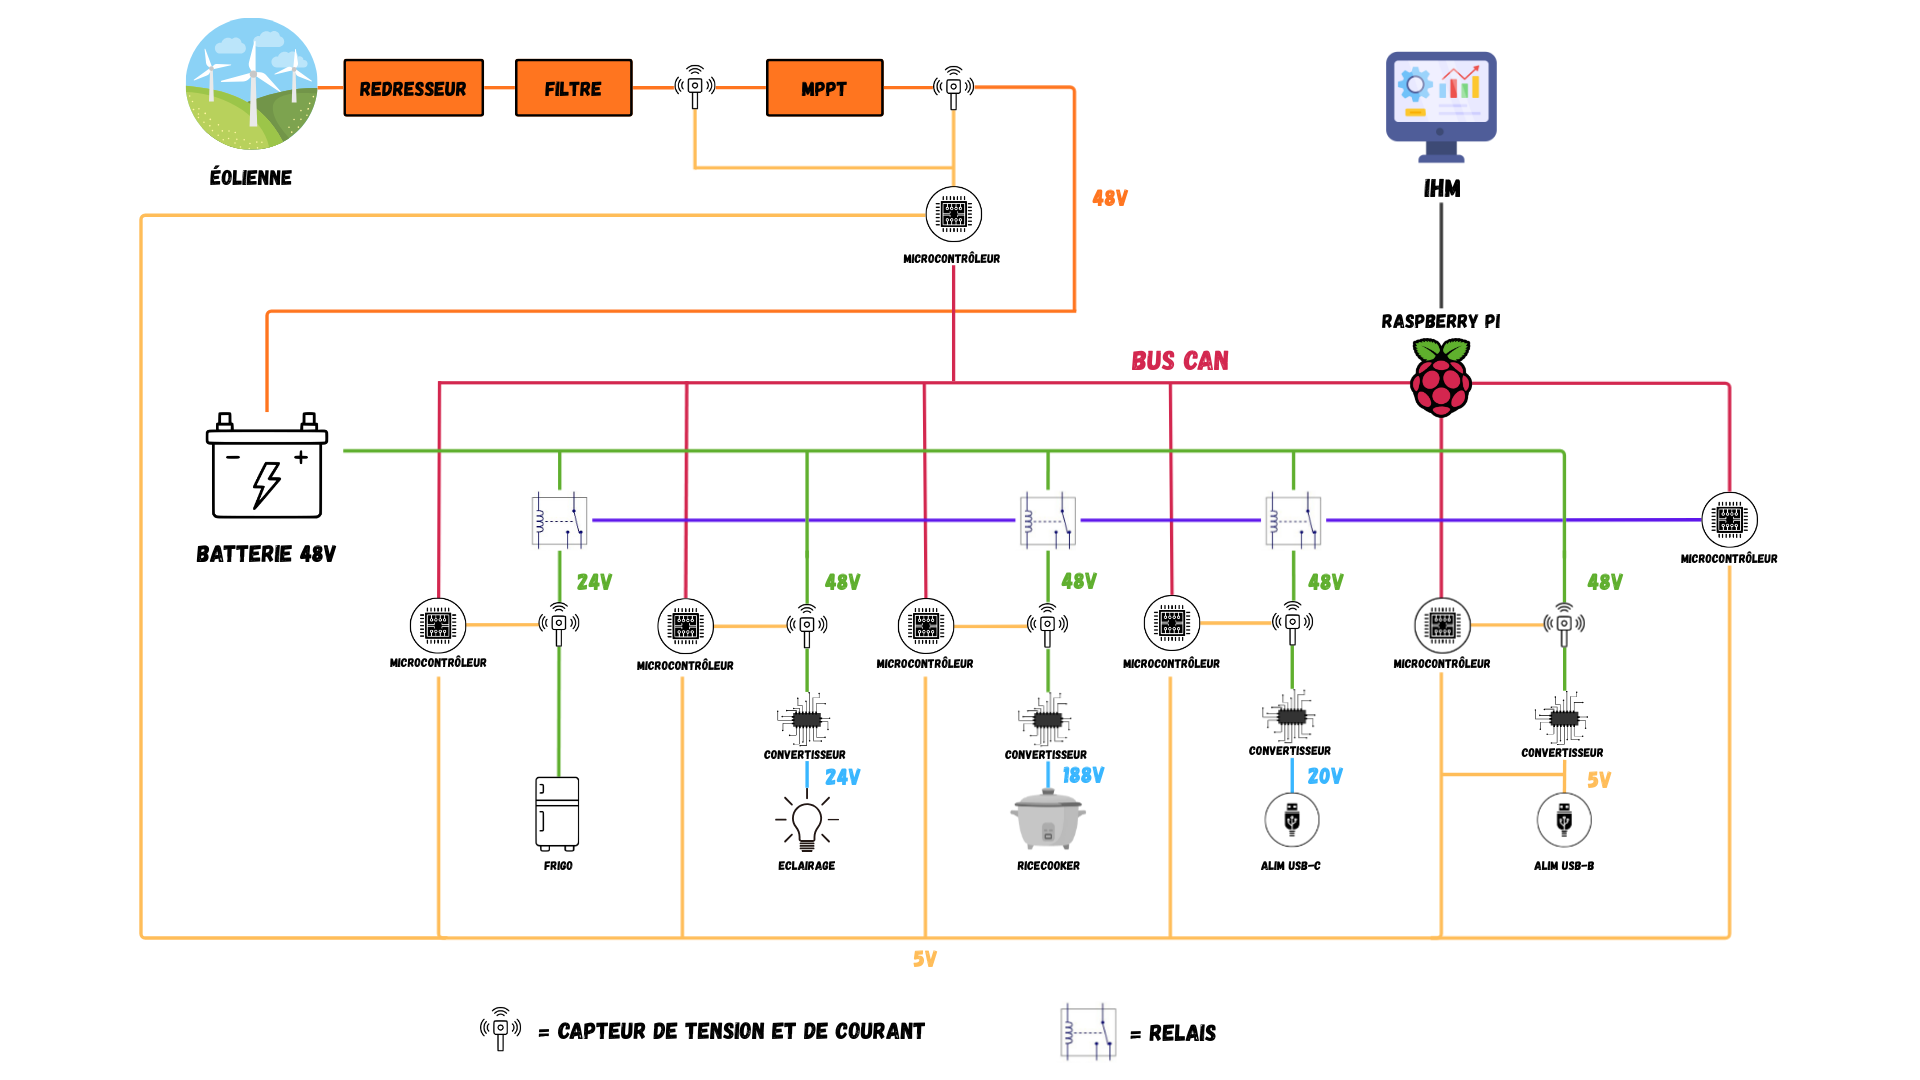
\includegraphics[width=0.9\textwidth]{images/diagrammes/Synoptique projet S8.png}
    \caption{Synoptique du Projet S8}
    \label{fig:synoptique}
\end{figure}

\section*{Organisation de l'équipe}
L'organisation de l'équipe pour ce semestre est présentée ci-dessous :
\begin{figure}[H]
    \centering
    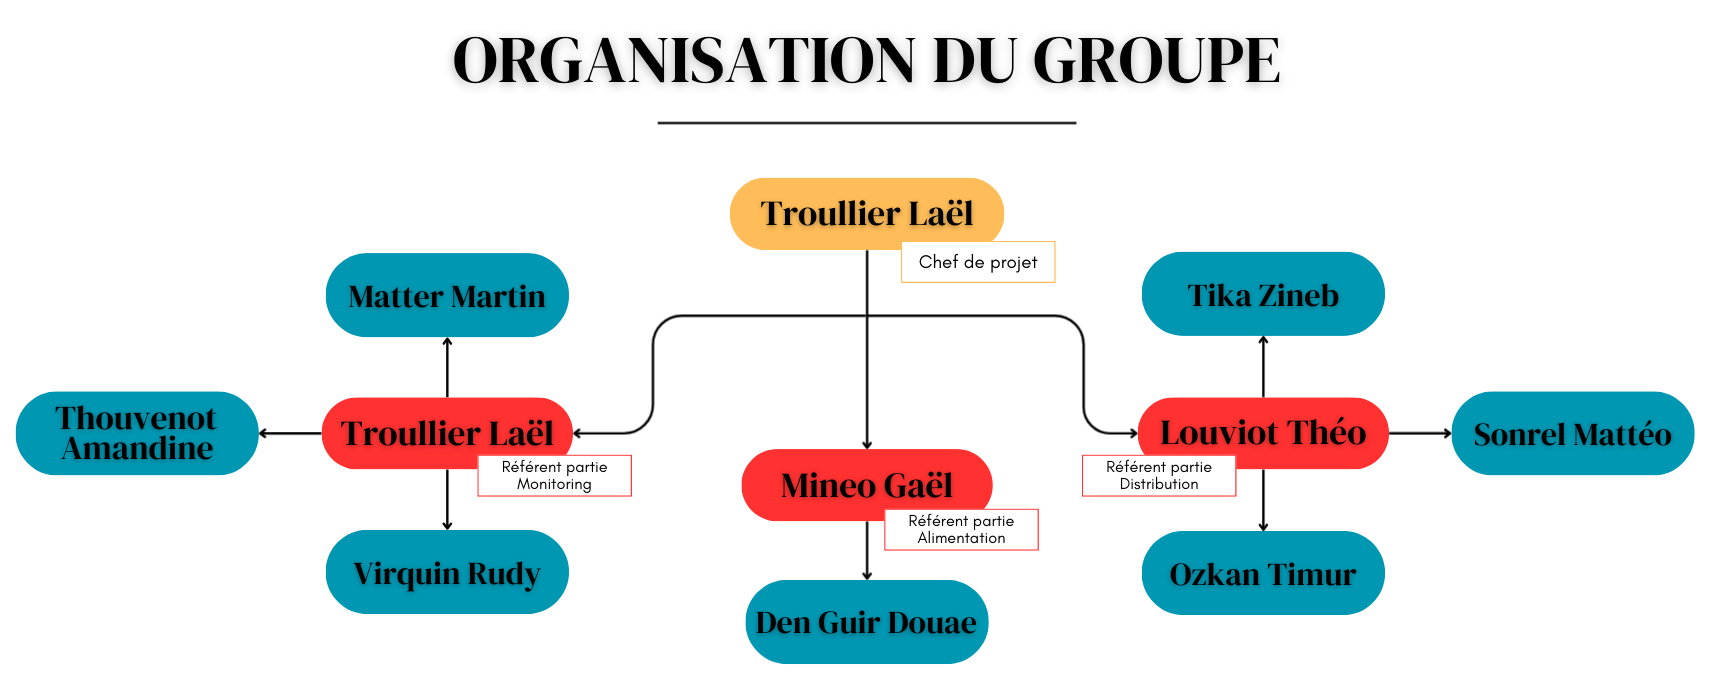
\includegraphics[width=0.9\textwidth]{images/diagrammes/Organigramme Projet S8.png}
    \caption{Organigramme du Projet S8}
    \label{fig:organigramme}
\end{figure}
\newpage
\tableofcontents
\newpage
\listoffigures
\newpage
% --- Planning du projet ---
\chapter{Plannification et Organisation}

\section{Planning prévisionnel}

Pour mener à bien le projet ce semestre, nous avons établi un planning prévisionnel détaillé basé sur les contraintes académiques et les jalons de rendus. Ce diagramme présente la répartition temporelle des tâches pour l'ensemble du groupe.

\begin{figure}[H]
    \centering
    \begin{ganttchart}[
        vgrid,
        hgrid,
        x unit=1.2cm,
        y unit title=0.8cm,
        y unit chart=0.6cm,
        title label font=\scriptsize\bfseries,
        bar label font=\tiny,
        group label font=\scriptsize\bfseries,
        milestone label font=\tiny\itshape
    ]{6}{23}
    
    % --- Titres des colonnes (Semaines) ---
    \gantttitle{Semaines du Semestre (S6 à S23)}{18} \\
    \gantttitlelist{6,...,23}{1} \\

    % --- SECTION 1 : GESTION & RENDUS ---
    \ganttgroup{Jalons \& Rendus}{6}{23} \\
    \ganttbar{Répartition des tâches}{6}{9} \\
    \ganttmilestone[milestone/.append style={fill=red}]{Rapport 1 (02/03)}{10} \\
    \ganttmilestone[milestone/.append style={fill=red}]{Rapport 2 (27/04)}{18} \\
    \ganttmilestone[milestone/.append style={fill=red}]{Rapport Final (05/06)}{23} \\

    % --- SECTION 2 : TACHES TECHNIQUES ---
    \ganttgroup{Node Red Solution (Rudy, Amandine)}{10}{22} \\
    \ganttbar{Développement solution}{10}{17} \\
    \ganttbar{Tests de communication}{19}{22} \\
    
    \ganttgroup{Alimentations \& Tests (?)}{6}{22} \\
    \ganttbar{Analyse \& CdC détaillé (?) }{6}{9} \\
    \ganttbar{Simulations, Schémas, PCB (?) }{10}{17} \\
    \ganttbar{Commande composants (?) }{12}{14} \\
    \ganttbar{Réalisation montage \& Validation (?) }{19}{22} \\

    % --- SECTION 3 : PERIODES SPECIALES ---
    \ganttbar[bar/.append style={fill=gray!30}]{Vacances / Examens}{16}{17}

    % Liens (dépendances simplifiées)
    \ganttlink{elem1}{elem2} 
    \ganttlink{elem2}{elem5} 
    
    \end{ganttchart}
    \caption{Diagramme de Gantt prévisionnel du projet S8}
    \label{fig:gantt_projet}
\end{figure}

\section{Organisation de l'équipe}
L'organisation de l'équipe pour ce semestre est présentée ci-dessous :
\begin{figure}[H]
    \centering
    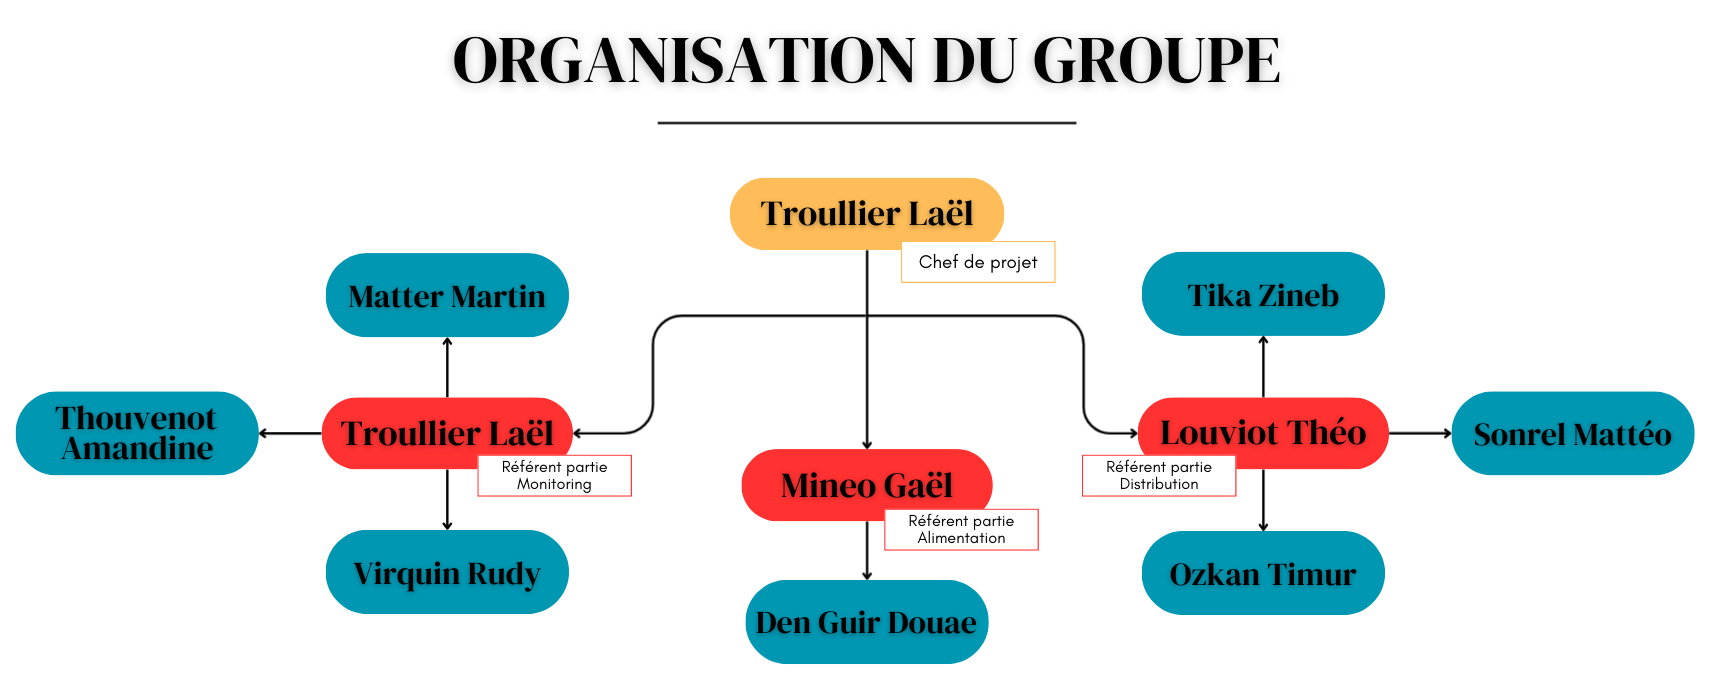
\includegraphics[width=1\textwidth]{images/diagrammes/Organigramme Projet S8.png}
    \caption{Organigramme du Projet S8}
    \label{fig:organigramme}
\end{figure}
\newpage
\chapter{Analyse Fonctionnelle et Technique}
\label{chap:analyse_fonctionnelle}

\section{Analyse Fonctionnelle}

Pour comprendre l'objectif principal du projet nous avons réalisé une "bête à cornes" et un diagramme "pieuvre".

\subsection{Bête à cornes}
Le schéma "bête à cornes" permet d'expliquer simplement et facilement la mission du projet.
\begin{figure}[H]
    \centering
    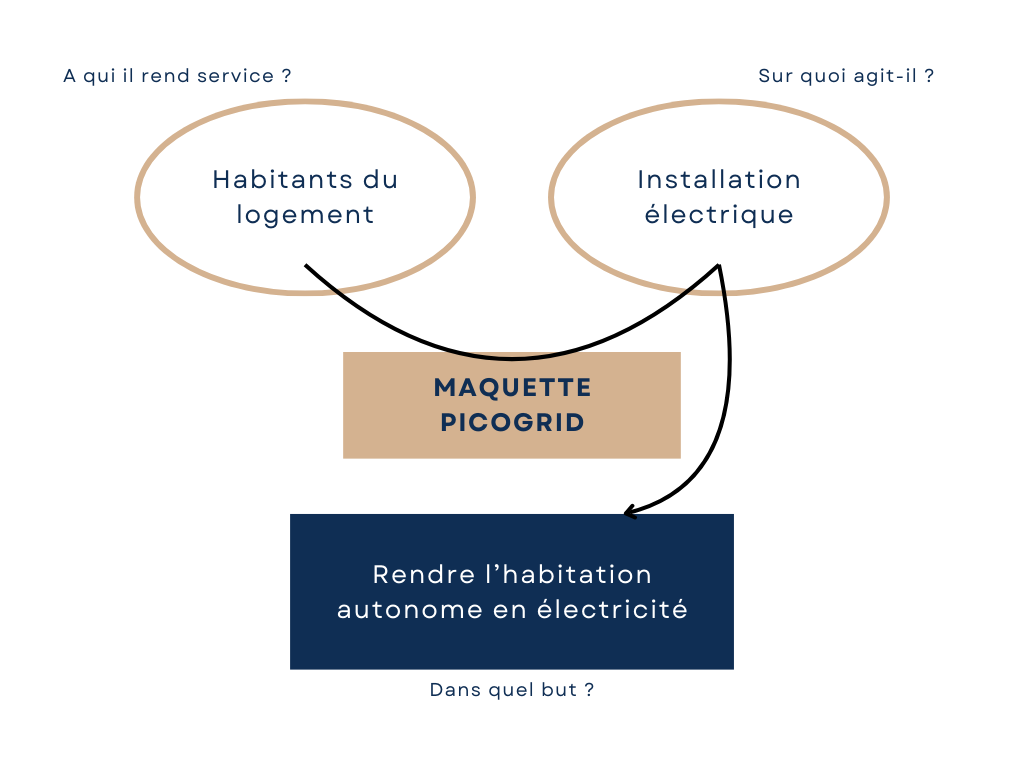
\includegraphics[width=0.8\textwidth]{images/diagrammes/Bête à cornes.png}
    \caption{Bête à cornes du projet}
    \label{fig:bete_a_cornes}
\end{figure}
Dans notre cas, la maquette Picogrid que nous allons réaliser est un dispositif conçu pour aider les habitants d'un logement à mieux gérer leur énergie. Son rôle est d'agir directement sur l'installation électrique de la maison afin de la rendre autonome. Ce système permet à l'habitation de produire et d'utiliser sa propre électricité, permettant son émancipation vis-à-vis du réseau électrique extérieur.

\subsection{Diagramme Pieuvre}
Le diagramme pieuvre permet de visualiser les fonctions de service du produit.
\begin{figure}[H]
    \centering
    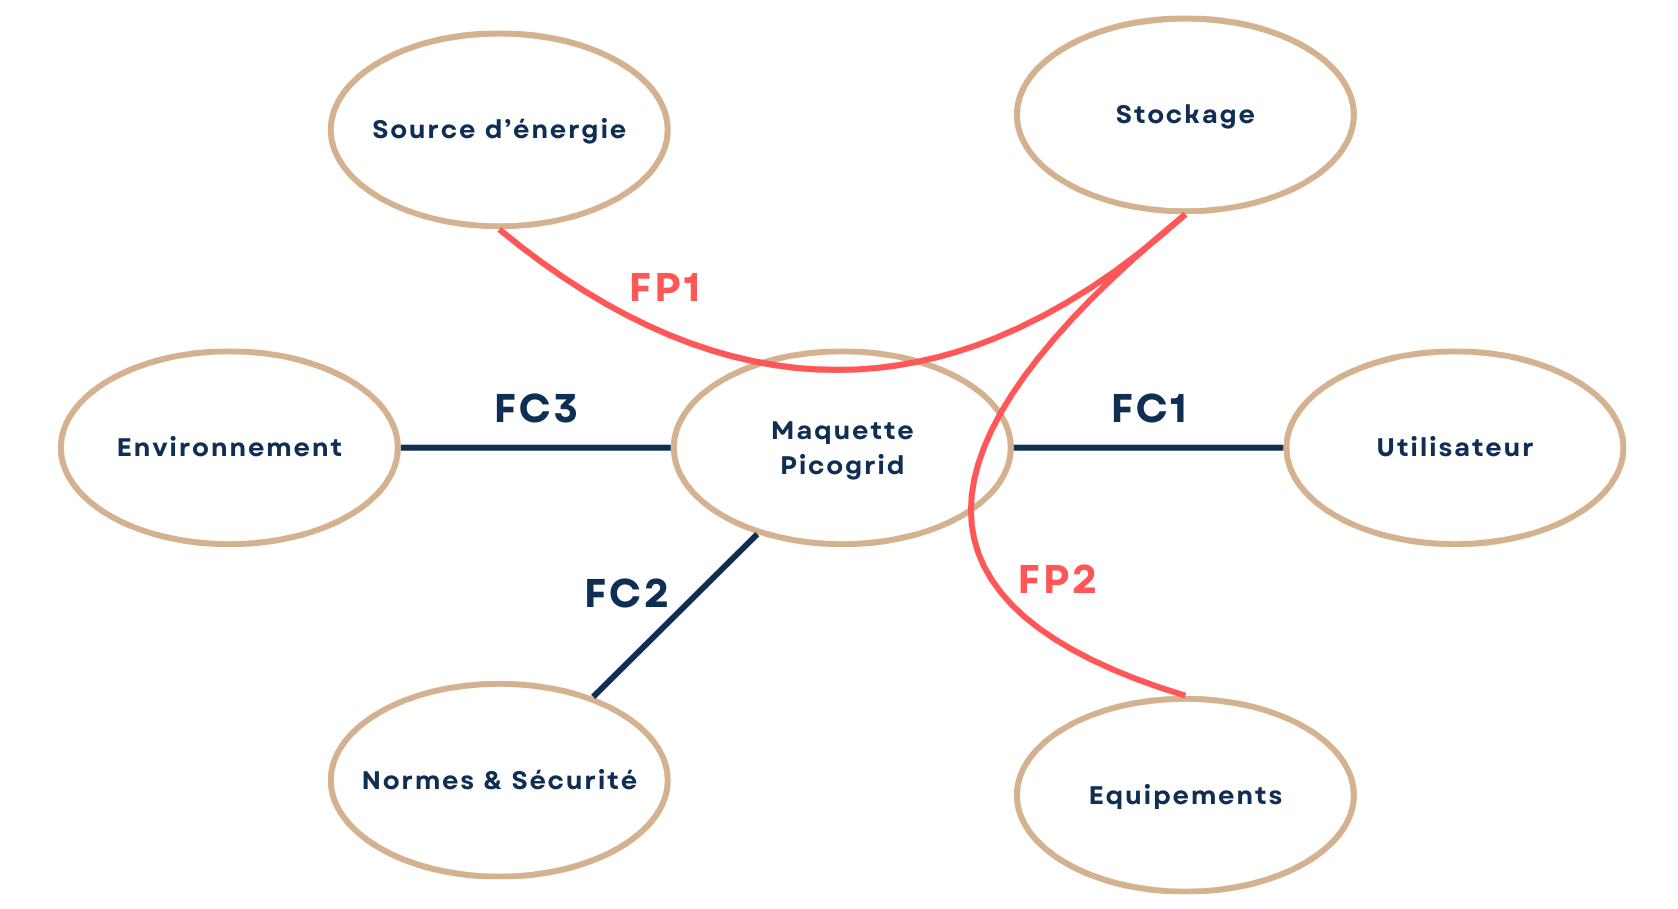
\includegraphics[width=0.8\textwidth]{images/diagrammes/Diagramme pieuvre.png}
    \caption{Diagramme Pieuvre du projet}
    \label{fig:pieuvre}
\end{figure}

\section{Rice Cooker}

\subsection{Caractéristiques Techniques du Rice Cooker}
\begin{itemize}
    \item \textbf{Puissance souhaitée} : 450\,W (contre 700\,W de base pour le fonctionnement normal du rice-cooker).
    \item \textbf{Nature de la charge} : Charge résistive et légèrement inductive. Une mesure réalisée au RLCmètre à 10\,kHz nous permet de trouver : $78\,\Omega$ et $10-11\,\mu H$.
    \item \textbf{Modulation} : L'alimentation doit être "modulable" pour faire varier la puissance de chauffe en fonction du mode désiré (cuisson et maintien en température).
    \item \textbf{Adaptation} : Fonctionnement en tension continue au lieu d'une tension alternative provenant du réseau (230\,Vac).
\end{itemize}

\subsection{Alimentation du Rice Cooker}
Le rice-cooker est un équipement qui permet de faire cuire du riz à l'aide d'une résistance qui va dissiper de la chaleur par effet Joule lors du passage d'un courant. C'est un équipement énergivore, donc on a limité sa puissance à 450\,W.

Son alimentation va nécessiter la création d'un convertisseur élévateur de tension continu (hacheur) avec les caractéristiques suivantes.

En supposant une tension d'entrée à 50\,V, on souhaite une puissance en sortie du convertisseur de 450\,W au maximum.

\subsubsection{Calcul du courant de sortie}
\begin{equation}
    I_s = \sqrt{\frac{P}{R}} = \sqrt{\frac{450}{78}} \approx 2,40\,\text{A}
\end{equation}
On en déduit la tension de sortie de notre convertisseur :
\begin{equation}
    V_s = \frac{P_s}{I_s} = \frac{450}{2,40} = 187,5\,\text{V}
\end{equation}

Donc le gain en tension de notre convertisseur devra être d'environ :
\begin{equation}
    G = \frac{V_s}{V_e} = \frac{187,5}{50} = 3,75
\end{equation}

Comme la puissance active est conservée (si on néglige les pertes dans le convertisseur), on obtient :
\begin{equation}
    P_s = P_e = 450\,\text{W}
\end{equation}
\begin{equation}
    I_e = \frac{V_s \times I_s}{V_e} = \frac{187,5 \times 2,40}{50} = 9\,\text{A}
\end{equation}

On aura donc un courant de 9\,A à l'entrée de notre convertisseur. Il faudra éventuellement prévoir un peu plus de puissance car il y aura des pertes dans le convertisseur. Les composants du hacheur ainsi que sa structure devront être choisis afin de respecter ces valeurs.

\subsection{Caractéristiques Techniques du Hacheur}
\begin{itemize}
    \item \textbf{Tension/courant d'entrée du convertisseur} : environ 50\,Vdc / 9\,A (voire un peu plus élevée quand les batteries sont chargées, batterie Plomb/Acide).
    \item \textbf{Tension/courant de sortie du convertisseur} : environ 187,5\,Vdc / 2,40\,A.
\end{itemize}

\section{Luminaires}

\subsection{Fonctions globales (Partie Puissance - Éclairage)}
\begin{itemize}
    \item Adapter la tension de la batterie (48\,V) aux besoins spécifiques du réseau d'éclairage.
    \item Distribuer l'énergie vers les 4 points d'éclairage LED définis (Cuisine, Salon, Coin lecture, Toilettes).
    \item Permettre l'allumage et l'extinction de chaque zone d'éclairage de manière manuelle et indépendante.
    \item Protéger matériellement les circuits d'éclairage contre les surintensités.
\end{itemize}

\subsection{Conversion d'énergie pour l'éclairage}
Le système doit être capable de transformer la tension continue issue de la batterie de stockage principale (plage de 42\,V à 56\,V) en une tension stable et sécurisée pour les luminaires de la maquette.

Pour cela nous devons mettre en place :
\begin{itemize}
    \item Un convertisseur DC/DC industriel du commerce abaissant la tension de la batterie (48\,V) vers un réseau 24\,V DC. Ce choix technologique présente un double avantage : il standardise le réseau secondaire avec les autres équipements de l'habitat (notamment le réfrigérateur), et il réduit significativement l'intensité du courant dans les câbles, minimisant ainsi les pertes par effet Joule.
\end{itemize}

Un dimensionnement optimisé pour une consommation totale inférieure à 20\,W, répartie de la manière suivante selon le besoin lumineux des pièces :
\begin{itemize}
    \item \textbf{Cuisine} : $\approx 6$\,W (Éclairage de travail fort)
    \item \textbf{Salon} : $\approx 5$\,W (Éclairage d'ambiance moyen)
    \item \textbf{Toilettes} : $\approx 3$\,W
    \item \textbf{Coin lecture} : $\approx 2$\,W (Éclairage minimal)
\end{itemize}
(Total estimé : $\approx 16$\,W, ce qui laisse une marge de sécurité technique pour le convertisseur).

\subsection{Distribution et commande de l'éclairage}
L'installation doit permettre un contrôle simple et direct par l'utilisateur. Ainsi le circuit de distribution doit comporter des interrupteurs mécaniques classiques sont placés sur chaque ligne pour contrôler les 4 zones séparément.

\section{Réfrigérateur}

\subsection{Fonctions globales (Partie Puissance - Réfrigération)}
\begin{itemize}
    \item Alimenter le réfrigérateur à partir du réseau de distribution continu adapté (24\,V).
    \item Assurer la production de froid de manière autonome.
\end{itemize}

\subsection{Caractéristiques de l'équipement}
D'après la plaque signalétique du réfrigérateur, les spécifications électriques requises sont :
\begin{itemize}
    \item \textbf{Tension d'entrée} : 12/24\,V d.c.
    \item \textbf{Puissance nominale} : 42\,W
\end{itemize}

\subsection{Tests et analyse de consommation}
Afin de valider le comportement électrique réel du compresseur sous 24\,V, nous avons effectué des mesures de courant :
\begin{itemize}
    \item \textbf{Régime transitoire (Démarrage)} : Lors de la mise en route, on relève un appel de courant générant un pic à 8\,A maximum.
    \item \textbf{Régime permanent} : Une fois la vitesse stabilisée, la consommation mesurée en continu s'établit à 1,4\,A.
\end{itemize}

\section{Distribution Ports USB}

\subsection{Fonctions globales (Partie Puissance)}
La partie distribution USB a pour objectif d'alimenter les équipements basse tension de l'installation à partir du bus batterie 48\,V.

Elle doit :
\begin{itemize}
    \item Adapter la tension 48\,V aux niveaux requis par les normes USB.
    \item Fournir une alimentation stable et sécurisée.
    \item Permettre la mesure de courant et tension pour le monitoring.
    \item Permettre le délestage en cas de batterie faible.
\end{itemize}

\subsection{USB-B (5V/2A)}
\subsubsection{Caractéristiques techniques}
La tension réelle du bus varie donc entre 42\,V et 56\,V, les convertisseurs DC-DC doivent être dimensionnés pour fonctionner sur toute cette plage.
\begin{itemize}
    \item \textbf{Tension de sortie} : 5\,V DC
    \item \textbf{Courant nominal minimal} : 2\,A (norme USB classique)
    \item \textbf{Puissance maximale estimée} : $P = 5\,\text{V} \times 2\,\text{A} = 10\,\text{W}$
\end{itemize}

\subsubsection{Conversion d'énergie}
La conversion 48\,V $\rightarrow$ 5\,V sera réalisée par un convertisseur DC-DC abaisseur (Buck synchrone).

\subsection{USB-C (20V/5A)}
\subsubsection{Caractéristiques techniques}
\begin{itemize}
    \item \textbf{Tension de sortie} : 20\,V DC
    \item \textbf{Courant maximal} : 5\,A
    \item \textbf{Puissance maximale} : 100\,W
\end{itemize}

\subsubsection{Conversion d'énergie}
La conversion 48\,V $\rightarrow$ 20\,V sera réalisée par un convertisseur DC-DC abaisseur.

\section{Monitoring}
Afin de pouvoir contrôler, monitorer et réguler l'ensemble de l'installation, il est fondamental de pouvoir mesurer avec précision les grandeurs électriques (tension et courant) à des points clés du circuit.

Ces données sont cruciales pour calculer la puissance produite par l'éolienne, la consommation de chaque équipement et l'état de charge de la batterie, permettant ainsi d'assurer le pilotage intelligent du système et le délestage des charges si nécessaire.

\subsection{Relevé des grandeurs électriques du système}
Le système doit être capable de connaître différentes valeurs de courant et tension en temps réel, et cela pour chaque équipement de l'installation électrique.
Pour cela nous devons mettre en place pour chaque convertisseur :
\begin{itemize}
    \item Un dispositif permettant de capter un niveau de courant;
    \item Un dispositif permettant de capter un niveau de tension.
\end{itemize}

Chaque convertisseur est associé à un dispositif de l'installation. Ainsi, nous aurons 6 convertisseurs pour les dispositifs suivants :
\begin{itemize}
    \item Frigo
    \item Rice cooker
    \item Éclairage
    \item USB-B
    \item USB-C
    \item Circuits électroniques
\end{itemize}

\subsection{Traitement et analyse des données}
Le système doit pouvoir traiter les données mesurées à chaque instant. Il doit être capable d'utiliser des valeurs de tension et courant pour déterminer des valeurs de :
\begin{itemize}
    \item La puissance générée par l'éolienne;
    \item La consommation de chaque équipement;
    \item L'état de charge de la batterie;
    \item Le temps restant estimé d'utilisation par équipement.
\end{itemize}

\subsection{Communication entre les dispositifs}
Les composants programmables (la Raspberry et les autres microcontrôleurs) présents dans le système doivent être en capacité de se transmettre des données. Il faut donc que chaque composant soit relié.
\newpage
\chapter{Cahier des charges détaillé}
\label{chap:cdc_detaille}

Ce chapitre détaille les spécifications techniques du projet, en se basant sur les éléments imposés et l'architecture retenue. L'analyse est structurée autour des trois sous-systèmes principaux : l'alimentation (production et stockage), la distribution (consommation) et le monitoring (pilotage et supervision).

\section{Éléments imposés}

Le projet s'articule autour d'un ensemble de matériels et de contraintes techniques imposés, qui définissent le cadre de l'étude :

\begin{itemize}
    \item \textbf{Source d'alimentation renouvelable} : Alternateur d’éolienne.
    \item \textbf{Conversion de puissance} : Convertisseur MPPT pour l'optimisation de la charge batterie.
    \item \textbf{Stockage} : Batterie plomb/acide 48\,V - 200\,Ah.
    \item \textbf{Charges} :
    \begin{itemize}
        \item 4 points d’éclairage LED.
        \item Une prise USB standard (5\,V / 2\,A).
        \item Une prise USB-C Power Delivery (20\,V / 5\,A).
        \item Alimentation 24\,V pour le réfrigérateur.
        \item Alimentation modulable 450\,W pour le rice-cooker.
    \end{itemize}
    \item \textbf{Auxiliaires} : Alimentations stabilisées pour l'électronique de commande (15\,V, 5\,V, 3,3\,V).
    \item \textbf{Pilotage et Interface} : Instrumentation sur bus CAN et application web de gestion temps réel.
\end{itemize}

\section{Partie 1 : Alimentation et Stockage}

Cette première partie traite de la conversion de l'énergie mécanique du vent en énergie électrique stockable. Elle englobe la chaîne de conversion depuis l'alternateur jusqu'à la batterie 48\,V.

\subsection{Source d'énergie : L'éolienne simulée}

La source d’alimentation repose sur une simulation en laboratoire. Un moteur asynchrone entraîne l’alternateur pour reproduire le comportement mécanique des pales d’une éolienne soumise au vent. Cette configuration permet de reproduire différentes vitesses de vent et d’analyser le comportement du système dans des conditions variées et maîtrisées.

L’énergie mécanique produite par le moteur est transmise à un alternateur. Celui-ci assure la conversion de l’énergie mécanique en énergie électrique sous forme de courant alternatif (AC), conformément au principe de fonctionnement d’une éolienne réelle.
À la sortie de l’alternateur, un redresseur AC/DC est mis en œuvre afin de convertir le courant alternatif en courant continu (DC). Cette étape est indispensable pour obtenir une tension continue exploitable, notamment en vue du stockage de l’énergie dans une batterie.

L’ensemble constitue ainsi une plateforme expérimentale permettant d’étudier et d’optimiser le fonctionnement d’un système éolien dans un environnement contrôlé.

\subsubsection{Caractérisation de l’alternateur}

\paragraph{Essai à vide}
L'essai à vide permet de caractériser la force électromotrice de la machine sans débit de courant, c'est-à-dire sans charge connectée,  afin d’analyser son comportement intrinsèque. Il permet notamment d’étudier la relation entre la vitesse de rotation et la tension de sortie. Les relevés confirment la nature triphasée des tensions (déphasage de $2\pi/3$) et montrent une relation linéaire entre la vitesse de rotation et la tension efficace, caractéristique des machines synchrones.

Pour l’ensemble de nos mesures, nous considérons une plage de vitesses comprise entre 500 et 750 tr/min. Pour chaque vitesse, nous relevons la tension efficace et la fréquence en sortie de l’alternateur.

\begin{tableau}[H]
    \centering
    \begin{tabularx}{0.8\textwidth}{X X X}
        \toprule
        \textbf{Vitesse (tr/min)} & \textbf{Fréquence (Hz)} & \textbf{Tension efficace (V)} \\
        \midrule
        500 & 50,2 & 133 \\
        1000 & 101,6 & 245 \\
        1500 & 150,7 & 358 \\
        \bottomrule
    \end{tabularx}
    \caption{Résultats de l'essai à vide de l'alternateur}
    \label{tab:essai_a_vide}
\end{tableau}

Le nombre de paires de pôles $p$ est déduit de la fréquence $f$ et de la vitesse $N$ :
\begin{equation}
    p = \frac{60 \cdot f}{N} = \frac{60 \cdot 50}{500} = 6 \quad \text{paires de pôles}
\end{equation}

\paragraph{Essai en charge}
L'essai en charge, permet d'évaluer le comportement du générateur en puissance. La tension alternative produite par l’alternateur est redressée au moyen d’un pont de diodes afin d’obtenir une tension continue. Une charge de type RL, composée d’une résistance et d’une inductance, est ensuite connectée en sortie du redresseur pour reproduire des conditions de fonctionnement proches d’une utilisation réelle.

\begin{figure}[H]
    \centering
    \begin{tikzpicture}[scale=1.0, thick]

% Left vertical line connecting the phases
\draw (0,2) -- (0,-2);

% --- Top phase ---
\draw (0,2) -- (0.5,2);
% Source E
\draw (1,2) circle (0.5);
\draw (0.5,2) -- (1.5,2);
\node at (1, 2.8) {$E$};
\draw (1.5,2) -- (2,2);
% Inductor lambda
\draw (2,2) arc (180:0:0.2) arc (180:0:0.2) arc (180:0:0.2) arc (180:0:0.2);
\node at (2.8, 2.6) {$\lambda$};
\draw (3.6,2) -- (4,2);
% Resistor r
\draw (4, 1.6) rectangle (5.2, 2.4);
\node at (4.6, 2.8) {$r$};
\draw (5.2,2) -- (6,2);

% --- Middle phase ---
\draw (0,0) -- (0.5,0);
% Source
\draw (1,0) circle (0.5);
\draw (0.5,0) -- (1.5,0);
\draw (1.5,0) -- (2,0);
% Inductor
\draw (2,0) arc (180:0:0.2) arc (180:0:0.2) arc (180:0:0.2) arc (180:0:0.2);
\draw (3.6,0) -- (4,0);
% Resistor
\draw (4, -0.4) rectangle (5.2, 0.4);
\draw (5.2,0) -- (6,0);

% --- Bottom phase ---
\draw (0,-2) -- (0.5,-2);
% Source
\draw (1,-2) circle (0.5);
\draw (0.5,-2) -- (1.5,-2);
\draw (1.5,-2) -- (2,-2);
% Inductor
\draw (2,-2) arc (180:0:0.2) arc (180:0:0.2) arc (180:0:0.2) arc (180:0:0.2);
\draw (3.6,-2) -- (4,-2);
% Resistor
\draw (4, -2.4) rectangle (5.2, -1.6);
\draw (5.2,-2) -- (6,-2);

% --- Rectifier block ---
\draw (6,-3) rectangle (10,3);
\node at (8, 3.4) {\large Redresseur};
\node at (6.5, 2.2) {\Large $\sim$};
\node at (9.2, 2.2) {\large PD3};

% Diode inside
\draw (7.2, 0) -- (7.6, 0);
\draw (7.6, 0.4) -- (7.6, -0.4) -- (8.4, 0) -- cycle;
\draw (8.4, 0.4) -- (8.4, -0.4);
\draw (8.4, 0) -- (8.8, 0);

% --- Output side ---
\draw (10, 1.8) -- (12.5, 1.8);
\draw (10, -1.8) -- (12.5, -1.8);

% Voltage arrow
\draw[-{Stealth[length=3mm]}] (10.5, -1.5) -- (10.5, 1.5);
\node[right] at (10.5, 0) {$V_{CH}$};

% --- Load block ---
\draw[blue, thick] (11.5, -1.6) rectangle (13.5, 1.2);
\node[right, blue] at (13.8, 0) {\large Charge RL};

% Load components
\draw (12.5, 1.8) -- (12.5, 0.8);
% Variable resistor R
\draw (12.1, 0.2) rectangle (12.9, 0.8);
\draw[-{Stealth[length=2mm]}] (11.8, 0) -- (13.2, 1.0);
\node[right] at (12.9, 0.5) {$R$};
\draw (12.5, 0.2) -- (12.5, -0.2);
% Inductor L
\draw (12.5, -0.2) arc (90:-90:0.2) arc (90:-90:0.2) arc (90:-90:0.2);
\node[right] at (12.7, -0.8) {$L$};
\draw (12.5, -1.4) -- (12.5, -1.8);

\end{tikzpicture}
    \caption{Schéma du montage expérimental pour l'essai en charge de l'alternateur}
    \label{fig:montage_test_charge}
\end{figure}

Comme illustré précédemment, des résistances de \SI{330}{\ohm} ont été utilisées afin de simuler une seule phase de l’alternateur et de permettre la mesure de la tension aux bornes de cette phase.
Les valeurs efficaces des tensions et des courants sont mesurées aux bornes de l’alternateur (côté AC) et à la sortie du redresseur (côté DC), ainsi que la fréquence électrique pour différentes vitesses de rotation et différentes valeurs de la résistance de charge R.
La puissance quant à elle à été trouvée à l’aide de la fonction MATH sur l'oscilloscope à l'aide de la tension mesurée aux bornes de la charge et le courant mesuré à l’aide d'une pince ampèremétrique.
Les résultats obtenus sont présentés dans les figures suivantes :

% insertion des 3 scopes

\begin{figure}[H]
    \centering
    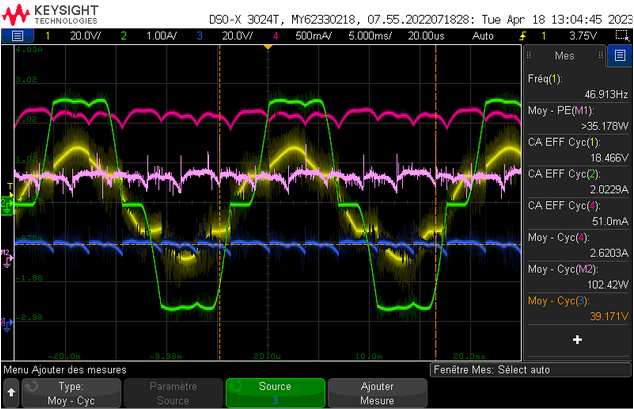
\includegraphics[width=0.8\textwidth]{images/scopes/Essai 500 trmin.png}
    \caption{Mesures à l’oscilloscope des grandeurs électriques de l’alternateur et du redresseur pour 500 tr/min}
    \label{fig:essai_500_trmin}
\end{figure}

\begin{figure}[H]
    \centering
    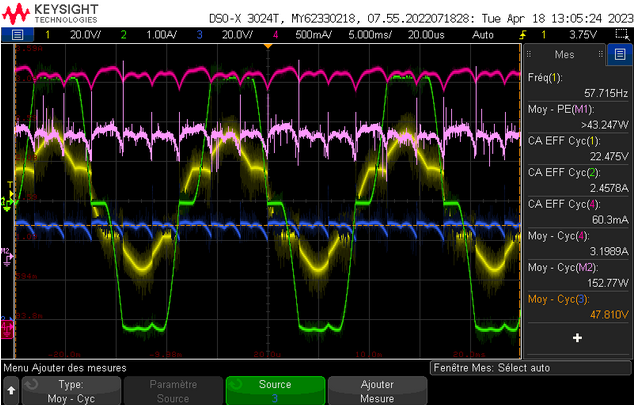
\includegraphics[width=0.8\textwidth]{images/scopes/Essai 600 trmin.png}
    \caption{Mesures à l’oscilloscope des grandeurs électriques de l’alternateur et du redresseur pour 600 tr/min}
    \label{fig:essai_600_trmin}
\end{figure}

\begin{figure}[H]
    \centering
    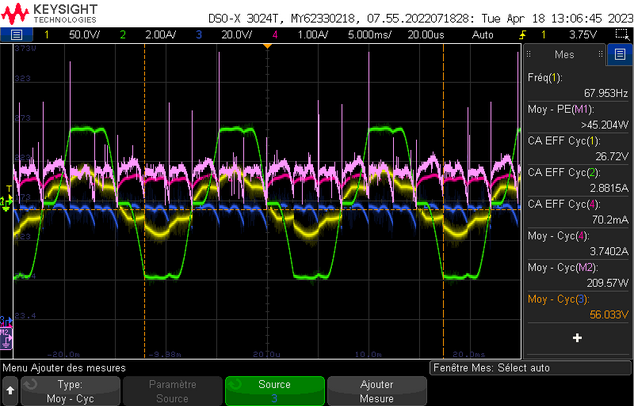
\includegraphics[width=0.8\textwidth]{images/scopes/Essai 700 trmin.png}
    \caption{Mesures à l’oscilloscope des grandeurs électriques de l’alternateur et du redresseur pour 700 tr/min}
    \label{fig:essai_700_trmin}
\end{figure}


Voici un résumé des résultats obtenus :

\begin{tableau}[H]
    \centering
    \begin{tabularx}{\textwidth}{X X X X X}
        \toprule
        \textbf{Vitesse (tr/min)} & \textbf{Fréq. (Hz)} & \textbf{Tension (V)} & \textbf{Courant (A)} & \textbf{Puissance (W)} \\
        \midrule
        500 & 46,9 & 39,2 & 2,62 & 102 \\
        600 & 57,7 & 47,8 & 3,20 & 153 \\
        700 & 67,9 & 56,0 & 3,74 & 210 \\
        \bottomrule
    \end{tabularx}
    \caption{Caractéristiques en charge après redressement}
    \label{tab:recap_charge}
\end{tableau}

Nous connaissons les caractéristiques  nominales de l’alternateur qui sont de 300W pour 750 tours/min, cependant lors de l’essai à 750 tr/min ce dernier n’a pas pu être mené à son terme. Sous charge, le moteur asynchrone d’entraînement ne parvenait pas à maintenir la vitesse nominale et calait immédiatement. Ce problème à empêché toute acquisition de mesures exploitables dans cette condition de fonctionnement.

\subsubsection{Modélisation de la source}
Pour concevoir le convertisseur MPPT, il est nécessaire de connaître l'impédance interne de la source (inductance de fuite). Celle-ci est déterminée en deux étapes à partir de l'observation de l'empiètement lors du redressement.

\paragraph{Calcul de l'empiètement}
L'empiètement $\mu$ est calculé à partir du temps de commutation des diodes observé à l'oscilloscope :
\begin{equation}
    \mu = 2 \cdot \pi \cdot f \cdot t_{com}
\end{equation}
où $f$ est la fréquence électrique et $t_{com}$ le temps de commutation.

\paragraph{Calcul de l'inductance interne}
À partir de l'empiètement $\mu$, l'inductance interne $\lambda$ est déduite à l'aide de la relation suivante :
\begin{equation}
    1 - \cos(\mu) = \frac{\lambda \cdot \omega \cdot I_{ch}}{V_s \cdot \sqrt{2} \cdot \sin(\pi/n)}
\end{equation}
D'où l'expression de l'inductance :
\begin{equation}
    \lambda = \frac{(1 - \cos\mu) \cdot V_s \cdot \sqrt{2} \cdot \sin(\pi/n)}{\omega \cdot I_{ch}}
\end{equation}

\textit{Note : Des mesures complémentaires sur oscilloscope sont encore nécessaires pour valider précisément le temps de commutation $t_{com}$ et finaliser la caractérisation de la source d’alimentation.}

\subsection{Convertisseur AC/DC (Redresseur)}
L'alternateur fournit en sortie une tension alternative, alors que le système nécessite une tension continue. Les redresseurs, qui assurent la transformation de l'énergie alternative en énergie continue, constituent l'une des solutions les plus courantes parmi les convertisseurs statiques. Cette conversion est essentielle pour obtenir une source de tension continue à partir de l'alimentation alternative.

Il existe principalement deux grandes catégories de redresseurs : non commandés et commandés.

Le choix final du redresseur dépend de la caractérisation complète de la source d'énergie et de la charge, étape désormais achevée et fournissant toutes les données nécessaires. Une analyse fonctionnelle et une étude bibliographique permettront d'identifier puis de sélectionner les deux ou trois solutions les plus pertinentes, qui seront ensuite simulées pour en valider les performances. La solution retenue sera dimensionnée, testée et validée avant fabrication, assurant un convertisseur fiable et parfaitement adapté à l'application.

\subsection{Gestion de la batterie et MPPT}
\label{sec:gestion_batterie}

Le stockage de l'énergie est assuré par un parc de batteries 48\,V, agissant comme tampon entre la production intermittente et la consommation.

\subsubsection{Caractéristiques du parc batterie}
Pour permettre de dimensionner correctement chaque convertisseur, il est important de bien comprendre le fonctionnement du parc de batteries, et plus particulièrement l'évolution des niveaux de tension en fonction de l'état de charge.
Les premières mesures réalisées au voltmètre aux bornes de chaque batterie au repos ont révélé des tensions aux alentours de 12,2\,V. En mettant ces 4 batteries en série, une tension réelle d'environ 48,8\,V est obtenue.
Le parc est donc constitué de 4 batteries 12\,V Plomb/Acide (200\,Ah) en série. Pour la suite du projet, il est crucial de garder à l'esprit que l'appellation « 48\,V » n'est qu'une valeur nominale. En pratique, la tension réelle varie significativement selon l'état de charge (SoC en anglais, pour State Of Charge) et le régime de fonctionnement, ce qui implique que tout le matériel connecté devra s'y adapter. Voici les principaux comportements à anticiper :

\begin{itemize}
    \item \textbf{La tension maximale lors de la recharge} : Pour “forcer” l'énergie à entrer dans une batterie, le chargeur doit appliquer une tension supérieure à la tension naturelle de celle-ci. Une batterie de 12\,V est composée de 6 cellules internes. Si une cellule pleine au repos délivre environ 2,1\,V ($6 \times 2,1 = 12,6\,\text{V}$), la chimie du plomb exige d'appliquer une tension d'environ 2,4\,V par cellule pour la recharger efficacement. Mathématiquement, la tension de charge atteint donc $6 \times 2,4 = 14,4\,\text{V}$ par batterie. Pour le parc de 4 éléments en série, la tension globale s'élève à $4 \times 14,4 = 57,6\,\text{V}$. Les convertisseurs devront impérativement être capables de supporter cette hausse (jusqu'à près de 58\,V) sans dommage.
    \item \textbf{La tension minimale de sécurité} : À l'inverse, pour éviter une dégradation irréversible des batteries (décharge profonde), le système de contrôle global devra couper l'alimentation vers les convertisseurs si la tension chute de manière critique (en dessous des seuils de sécurité indiqués dans le tableau ci-dessous).
    \item \textbf{La chute de tension en utilisation (sous charge)} : Il est important de ne pas confondre une batterie « en charge » et une batterie « sous charge » (qui alimente le système). Dès l'allumage de l'ensemble des équipements électriques, l'effort demandé fait artificiellement chuter la tension mesurée aux bornes des batteries en raison de leur résistance interne. Lors de la programmation, il faudra bien distinguer cette baisse de tension normale liée à l'utilisation d'une véritable batterie déchargée. Le système devra toutefois être capable d'estimer le niveau d'énergie restant en temps réel à partir des valeurs de référence suivantes.
\end{itemize}

\begin{tableau}[H]
    \centering
    \begin{tabularx}{\textwidth}{X l l X}
        \toprule
        \textbf{État de charge} & \textbf{Tension (12\,V)} & \textbf{Tension (48\,V)} & \textbf{État de la batterie} \\
        \midrule
        100\% & 12,6\,V - 12,7\,V & 50,4\,V - 50,8\,V & Charge complète \\
        80\% & 12,4\,V & 49,6\,V & Bon état \\
        60\% & 12,2\,V & 48,8\,V & Partiellement déchargée \\
        40\% & 11,9\,V & 47,6\,V & Décharge critique \\
        20\% & 11,6\,V & 46,4\,V & Décharge profonde (Dégâts matériels) \\
        10\% ou moins & 11,3\,V ou moins & 45,2\,V ou moins & Batterie potentiellement hors d’usage \\
        \bottomrule
    \end{tabularx}
    \caption{État de charge des batteries en fonction de la tension à vide}
    \label{tab:batterie_soc_new}
\end{tableau}

\subsubsection{Convertisseur DC/DC et Stratégie MPPT}

Étant donné que la tension continue issue du pont redresseur varie fortement en fonction de la vitesse de rotation de l’alternateur (elle-même dépendante des fluctuations du vent simulé), il est indispensable d’intégrer un convertisseur DC/DC commandé par un algorithme MPPT. Le MPPT, de l'anglais Maximum Power Point Tracking, a pour objectif de maximiser en permanence la puissance extraite de la source, en s’assurant que le système fonctionne toujours au point de puissance maximal. \\
Ce convertisseur a un double rôle : Adapter dynamiquement l’impédance vue par l’alternateur afin d’extraire la puissance maximale disponible et convertir la tension redressée variable en une tension compatible avec la charge d’une batterie 48 V.

\section{Partie 2 : Distribution et Charges}
\label{sec:distribution}

Cette partie détaille l'ensemble des équipements connectés au bus 48\,V. Chaque charge nécessite une interface de puissance spécifique pour adapter la tension du bus aux besoins de l'application.

\subsection{Électroménager de puissance : Le Rice Cooker}
\label{subsec:rice_cooker}

L'intégration du rice-cooker au système nécessite une adaptation profonde de son alimentation d'origine afin de respecter les contraintes de puissance et de nature du réseau.

\subsubsection{Objectif d'adaptation et ergonomie}
L'objectif est de garantir une utilisation « transparente » pour l'utilisateur final. L'appareil, initialement conçu pour fonctionner en courant alternatif (230\,V$_{ac}$), doit être modifié pour s'intégrer à l'installation en courant continu. Il convient donc de s'assurer que l'ensemble des composants internes peuvent fonctionner sous la tension continue prévue sans dégradation de leurs fonctions.

\subsubsection{Caractéristiques techniques de la charge}
Les spécifications retenues pour le rice-cooker au sein du projet sont les suivantes :
\begin{itemize}
    \item \textbf{Puissance de fonctionnement} : Limitée à 450\,W (contre 700\,W d'origine).
    \item \textbf{Nature de la charge} : Charge majoritairement résistive avec une composante inductive mineure.
    \item \textbf{Mesures d'impédance} : Une caractérisation au RLCmètre à 10\,kHz a permis de mesurer une résistance $R = 78\,\Omega$ et une inductance $L \approx 10-11\,\mu$H.
    \item \textbf{Modulation de puissance} : L'alimentation doit être modulable afin de faire varier la puissance de chauffe selon le mode désiré (cuisson et maintien en température).
    \item \textbf{Adaptation} : Fonctionnement en tension continue au lieu d’une tension alternative provenant du réseau domestique (230\,V$_{ac}$).

\end{itemize}

\subsubsection{Alimentation du Rice Cooker}
Le rice-cooker est un équipement qui permet de faire cuire du riz à l’aide d’une résistance de qui va dissiper de la chaleur par effet Joule lors du passage d’un courant. C’est un équipement énergivore donc on a limité sa puissance à 450\,W. Son alimentation à partir du bus 48\,V, va nécessiter la création d’un convertisseur élévateur de tension continu (hacheur).
En considérant une tension d'entrée nominale $V_e = 50$\,V et une puissance de sortie maximale $P_s = 450$\,W, les grandeurs électriques sont déterminées comme suit :

Le courant de sortie requis pour la charge est de :
\begin{equation}
    I_s = \sqrt{\frac{P_s}{R}} = \sqrt{\frac{450}{78}} \approx 2,40\,\text{A}
\end{equation}

La tension de sortie du convertisseur doit donc être de :
\begin{equation}
    V_s = \frac{P_s}{I_s} = \frac{450}{2,40} = 187,5\,\text{V}
\end{equation}

Le gain en tension statique $G$ du convertisseur est alors :
\begin{equation}
    G = \frac{V_s}{V_e} = \frac{187,5}{50} = 3,75
\end{equation}

Sous l'hypothèse d'une conservation de la puissance active (en négligeant les pertes du convertisseur), la puissance d'entrée $P_e$ est égale à $P_s = 450$\,W. Le courant d'entrée moyen $I_e$ est alors :
\begin{equation}
    I_e = \frac{V_s \cdot I_s}{V_e} = \frac{187,5 \cdot 2,40}{50} = 9\,\text{A}
\end{equation}

En pratique, il convient de prévoir une marge de puissance supplémentaire pour compenser les pertes de conduction et de commutation du hacheur. Les composants de puissance et la structure du hacheur devront être dimensionnés pour supporter ces contraintes de courant (9\,A à l'entrée) et de tension (187,5\,V à la sortie).

\paragraph{Synthèse des caractéristiques techniques du hacheur}

Sur la base des calculs précédents, les spécifications techniques du convertisseur élévateur sont résumées comme suit :
\begin{itemize}
    \item \textbf{Grandeurs d'entrée} : environ 50\,V$_{dc}$ / 9\,A. Cette tension peut être légèrement plus élevée lorsque les batteries Plomb/Acide sont en fin de charge (jusqu'à 58\,V).
    \item \textbf{Grandeurs de sortie} : environ 187,5\,V$_{dc}$ / 2,40\,A.
\end{itemize}

\subsection{Éclairage domestique}

% insère une phrase d'introduction pour présenter le contexte de l'éclairage domestique dans la maquette et les besoins spécifiques liés à l'échelle réduite.


\subsubsection{Fonctions globales}
\begin{itemize}
    \item Adapter la tension de la batterie (48\,V) aux besoins spécifiques du réseau d'éclairage.
    \item Distribuer l'énergie vers les 4 points d'éclairage LED définis (Cuisine, Salon, Coin lecture, Toilettes).
    \item Permettre l'allumage et l'extinction de chaque zone d'éclairage de façon manuelle et indépendante.
    \item Protéger matériellement les circuits d'éclairage contre les surintensités.
\end{itemize}

\subsubsection{Conversion d'énergie pour l'éclairage}
Le système doit être capable de transformer la tension continue issue de la batterie de stockage principale (plage de 42\,V à 58\,V) en une tension stable et sécurisée pour les luminaires de la maquette. Pour cela nous devons mettre en place :
\begin{itemize}
    \item Un convertisseur DC/DC industriel du commerce abaissant la tension de la batterie (48\,V) vers un réseau 24\,V DC.
    \item Un dimensionnement optimisé pour une consommation totale inférieure à 20\,W. Ces puissances sont volontairement adaptées à l'échelle réduite de la maquette : elles suffisent amplement à reproduire les niveaux d'éclairement normés d'une vraie maison (en Lux) sans provoquer d'éblouissement sur une surface miniature. La puissance est répartie de la manière suivante selon le besoin lumineux des pièces :
    \begin{itemize}
        \item \textbf{Cuisine} : $\approx 6$\,W (Éclairage de travail fort).
        \item \textbf{Salon} : $\approx 5$\,W (Éclairage d'ambiance moyen).
        \item \textbf{Toilettes} : $\approx 3$\,W.
        \item \textbf{Coin lecture} : $\approx 2$\,W (Éclairage minimal).
    \end{itemize}
    (Total estimé : $\approx 16$\,W, ce qui laisse une marge de sécurité technique pour le convertisseur).
\end{itemize}

\subsubsection{Distribution et commande de l'éclairage}
L'installation doit permettre un contrôle simple et direct par l'utilisateur. Ainsi le circuit de distribution doit comporter :
\begin{itemize}
    \item Des interrupteurs mécaniques classiques placés sur chaque ligne pour contrôler les 4 zones séparément.
\end{itemize}

\subsection{Réfrigérateur}

\subsubsection{Fonctions globales}
\begin{itemize}
    \item Alimenter le réfrigérateur à partir du réseau de distribution continu adapté (24\,V).
    \item Assurer la production de froid de manière autonome.
\end{itemize}

\subsubsection{Caractéristiques de l'équipement}
D'après la plaque signalétique du réfrigérateur, les spécifications électriques requises sont :
\begin{itemize}
    \item \textbf{Tension d'entrée} : 12/24\,V$_{dc}$.
    \item \textbf{Puissance nominale} : 42\,W.
\end{itemize}

\subsubsection{Tests et analyse de consommation}
Afin de valider le comportement électrique réel du compresseur sous 24\,V, nous avons effectué des mesures de courant :
\begin{itemize}
    \item \textbf{Régime transitoire (Démarrage)} : Lors de la mise en route, on relève un appel de courant générant un pic à 8\,A maximum.
    \item \textbf{Régime permanent} : Une fois la vitesse du compresseur stabilisée, la consommation mesurée en continu s'établit à 1,4\,A.
\end{itemize}

\begin{figure}[H]
    \centering
    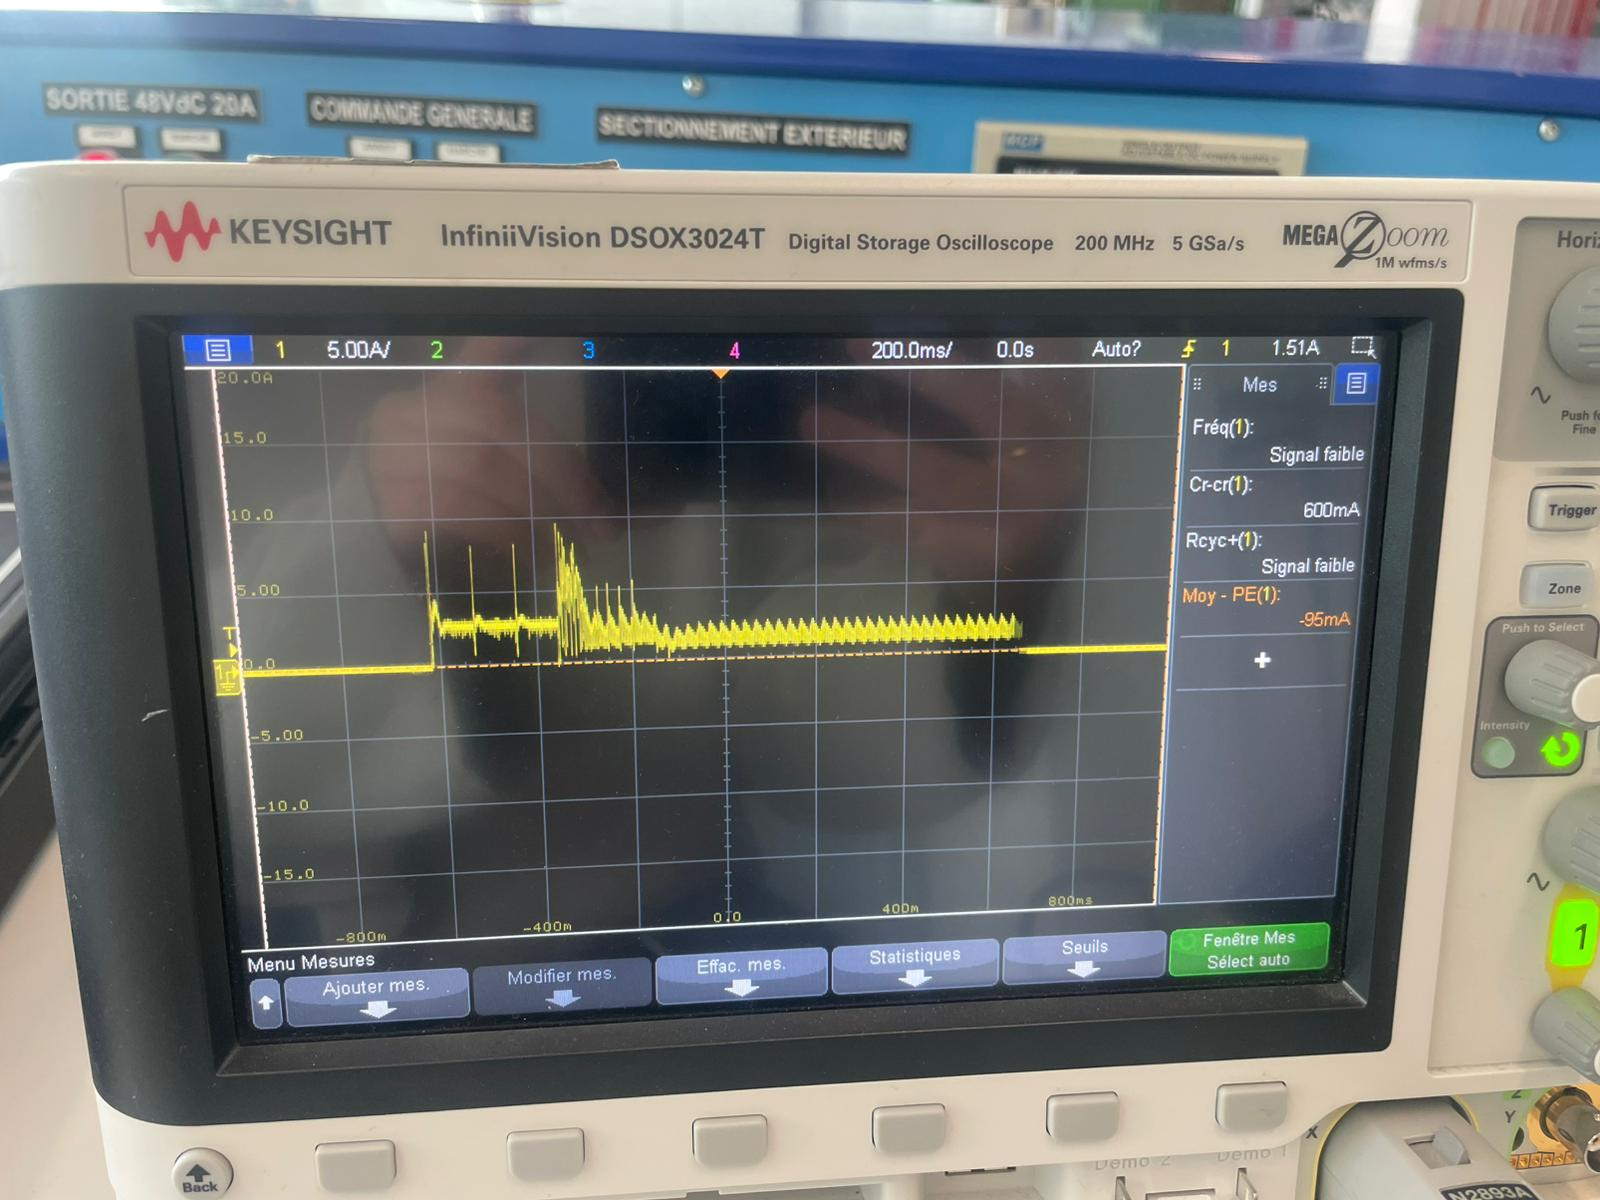
\includegraphics[width=0.8\textwidth]{images/scopes/scope refrigerateur.jpeg}
    \caption{Mesure à l’oscilloscope du courant de démarrage du réfrigérateur}
    \label{fig:scope_refrigerateur}
\end{figure}

Les protections devront être adaptées pour permettre au réfrigérateur de démarrer sans déclencher l’ouverture de son circuit d'alimentation.

\subsection{Distribution USB (Multimédia)}

L’intégration de ports USB au sein du système permet d’alimenter des équipements électroniques basse tension à partir du bus batterie 48\,V.
Aujourd’hui, les standards USB-B et USB-C sont devenus incontournables dans l’alimentation des dispositifs électroniques, qu’il s’agisse de périphériques classiques (5\,V) ou d’équipements nécessitant une puissance plus élevée via la norme USB-C Power Delivery (20\,V / 5\,A).

L’objectif de cette partie est donc d’assurer une conversion d’énergie fiable, efficace et sécurisée, tout en garantissant la compatibilité avec les normes électriques en vigueur.
La tension issue du pack batterie est nominalement de 48\,V, mais elle varie selon l’état de charge :
\begin{itemize}
    \item En fin de décharge $\approx 42$\,V
    \item En charge maximale $\approx 58$\,V
\end{itemize}
Les convertisseurs devront donc fonctionner correctement sur toute cette plage de tension.

La distribution USB doit répondre aux exigences suivantes :
\begin{itemize}
    \item Adapter la tension 48\,V aux niveaux requis par les normes USB (5\,V et 20\,V)
    \item Fournir une tension régulée avec une faible ondulation
    \item Garantir la protection contre les surtensions, surintensités et courts-circuits
    \item Permettre la mesure du courant et de la tension pour la partie monitoring
    \item Autoriser le délestage du port USB-C en cas de batterie faible afin de préserver l’autonomie du système
    \item Assurer un bon rendement énergétique pour limiter les pertes et l’échauffement
\end{itemize}
Cette architecture permet d’alimenter à la fois les dispositifs externes (prises USB) et certains systèmes internes de commande (Raspberry Pi, microcontrôleurs), tout en conservant une gestion centralisée de l’énergie.

\subsubsection{USB-B (5\,V / 7\,A)}
\paragraph{Caractéristiques et contraintes}
\begin{itemize}
    \item \textbf{Tension d’entrée} : 42\,V à 58\,V
    \item \textbf{Tension de sortie régulée} : 5\,V$_{dc}$
    \item \textbf{Tolérance} : conforme à la norme USB ($\pm 5\,\%$)
    \item \textbf{Courant nominal minimal} : 2\,A + 5\,A (Alimentation de la partie monitoring)
    \item \textbf{Puissance maximale estimée} : 35\,W
    \item \textbf{Stabilité} : Faible ondulation de sortie afin de garantir la stabilité des équipements électroniques sensibles
    \item \textbf{Protection contre} : les surtensions, les surintensités, les courts-circuits
    \item \textbf{Intégration} : dans l’architecture globale du système (montage industriel)
    \item \textbf{Supervision} : Possibilité de mesurer courant et tension pour le monitoring
\end{itemize}

\paragraph{Principe de conversion}
La tension du bus batterie (48\,V nominal) étant supérieure à la tension requise en sortie (5\,V), une conversion DC-DC abaisseuse est nécessaire afin d’adapter le niveau de tension tout en garantissant un bon rendement énergétique.
Un schéma bloc de la chaîne d’énergie est présenté ci-dessous :

\begin{figure}[H]
    \centering
    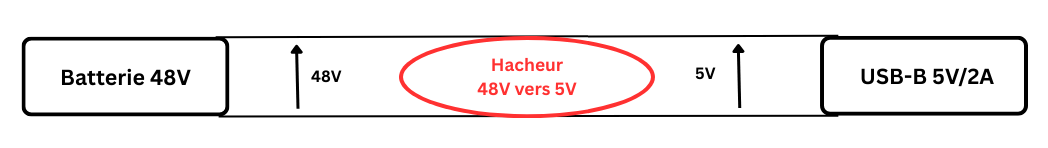
\includegraphics[width=0.8\textwidth]{images/figures/USB-B.png}
\end{figure}


\subsubsection{USB-C (20\,V / 5\,A)}
\paragraph{Caractéristiques et contraintes}
\begin{itemize}
    \item \textbf{Tension d’entrée} : 42\,V à 58\,V
    \item \textbf{Tension de sortie} : 20\,V$_{dc}$
    \item \textbf{Courant maximal} : 5\,A
    \item \textbf{Puissance maximale} : 100\,W
\end{itemize}
Les contraintes relatives à la stabilité de la tension, à la limitation d’ondulation, aux protections électriques (surtension, surintensité, court-circuit), à l’intégration mécanique ainsi qu’à la supervision énergétique sont identiques à celles décrites pour le convertisseur USB-B.

\paragraph{Principe de conversion}
Comme pour le port USB-B, l’adaptation de la tension du bus batterie vers la tension requise en sortie nécessite une conversion DC-DC abaisseuse. La chaîne d’énergie est donc la suivante :

\begin{figure}[H]
    \centering
    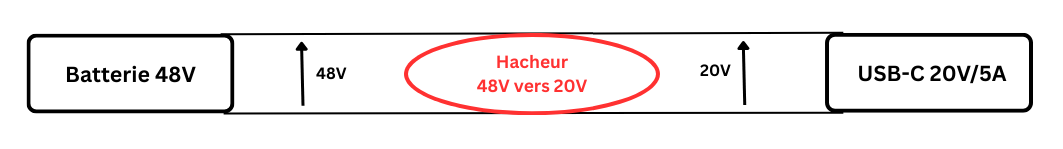
\includegraphics[width=0.8\textwidth]{images/figures/USB-C.png}
\end{figure}

\section{Partie 3 : Monitoring et Contrôle}
\label{sec:monitoring}

Le système de contrôle est le "cerveau" de l'installation. Il assure la sécurité, la gestion de l'énergie et l'interface utilisateur.
Afin de pouvoir contrôler, monitorer et réguler l’ensemble de l’installation, il est fondamental de pouvoir mesurer avec précision les grandeurs électriques (tension et courant) à des points clés du circuit. Ces données sont cruciales pour calculer la puissance produite par l’éolienne, la consommation de chaque équipement et l'état de charge de la batterie, permettant ainsi d’assurer le pilotage intelligent du système et le délestage des charges si nécessaire.

\subsection{Instrumentation - Relevé des grandeurs électriques du système}
Le système doit être capable de connaître différentes valeurs de courant et tension en temps réel, et cela pour chaque équipement de l’installation électrique. Pour cela nous devons mettre en place pour chaque convertisseur : 
\begin{itemize}
    \item Un dispositif permettant de capter un niveau de courant.
    \item Un dispositif permettant de capter un niveau de tension.
\end{itemize}

Voici l'ordre de grandeur des valeurs électriques que nous aurons à mesurer (données de dimensionnement des capteurs) : 

\begin{tableau}[H]
    \centering
    \begin{tabularx}{\textwidth}{X c c}
        \toprule
        \textbf{Convertisseur} & \textbf{Courant attendu (A)} & \textbf{Tension attendue (V)} \\
        \midrule
        USB-B & 7 & 5 \\
        USB-C & 5 & 20 \\
        Rice-cooker amont & 9 & 50 \\
        Rice-cooker aval & 2,40 & 187,5 \\
        Réfrigérateur & 8 (pic) / 1,4 (stabilisé) & 24 \\
        Éclairage & 0,85 & 24 \\
        MPPT amont & ??? & ??? \\
        MPPT aval & ??? & 48 \\
        \bottomrule
    \end{tabularx}
    \caption{Ordres de grandeur des mesures pour le monitoring}
    \label{tab:monitoring_values_detailed}
\end{tableau}

\subsection{Architecture de communication}
Les composants programmables présents dans le système doivent-être en capacité de se transmettre des données. Il faut donc que chaque composant soit relié aux autres. Le pilotage est distribué : chaque sous-ensemble (convertisseurs, capteurs) communique via un bus de terrain \textbf{CAN (Controller Area Network)}. Ce choix garantit la robustesse des échanges dans un environnement électriquement bruité (hacheurs de puissance). Le système devra donc comporter une gestion des priorités de communication. Les données collectées sont ensuite centralisées et traitées par un microcontrôleur ou un mini-ordinateur (ex : Raspberry Pi) qui assure la supervision globale du système.

\subsection{Traitement et analyse des données}
Le système doit pouvoir traiter les données mesurées à chaque instant. Il doit être capable d’utiliser des valeurs de tension et courant pour déterminer : 
\begin{itemize}
    \item La puissance générée par l’éolienne.
    \item La consommation de chaque équipement.
    \item L’état de charge de la batterie.
    \item Le temps restant estimé d’utilisation par équipement.
\end{itemize}

\subsection{Stratégie de délestage}
Afin de protéger la batterie contre les décharges profondes, le système supervise la tension du bus 48\,V. En cas de baisse critique, un délestage automatique est opéré selon un ordre de priorité défini :
\begin{enumerate}
    \item Rice-cooker (arrêt immédiat).
    \item Port USB-C (coupure).
    \item Réfrigérateur.
\end{enumerate}
L'éclairage et le système de monitoring restent alimentés le plus longtemps possible.

\subsection{Interface Homme-Machine (IHM)}
Le système doit permettre à l’utilisateur de visualiser les données acquises via une interface web, soit depuis un écran directement sur le dispositif de contrôle, soit par l’intermédiaire de tout navigateur web connecté au réseau internet de l’environnement.
Une application web, hébergée localement, permet à l'utilisateur de visualiser l'état du système selon deux modes d’affichage :



\begin{itemize}
    \item Un mode d’affichage \textbf{simplifié} pour l'utilisateur lambda avec des informations sur la charge globale du système, la production d’énergie et si l’énergie disponible permet d’utiliser les différents équipements.
    \item Un mode d’affichage \textbf{expert} indiquant toutes les mesures effectuées (tensions, courants, etc…) permettant un contrôle plus fin sur le système.
\end{itemize}

\end{document}
